%% LyX 2.1.4 created this file.  For more info, see http://www.lyx.org/.
%% Do not edit unless you really know what you are doing.
\documentclass[12pt,english]{article}
\usepackage[T1]{fontenc}
\usepackage[latin9]{inputenc}
\usepackage{geometry}
\geometry{verbose}
\setlength{\parskip}{\medskipamount}
\setlength{\parindent}{0pt}
\usepackage{graphicx}

\makeatletter

%%%%%%%%%%%%%%%%%%%%%%%%%%%%%% LyX specific LaTeX commands.
%% Because html converters don't know tabularnewline
\providecommand{\tabularnewline}{\\}

%%%%%%%%%%%%%%%%%%%%%%%%%%%%%% User specified LaTeX commands.
\usepackage[amssymb]{SIunits}

\makeatother

\usepackage{babel}
\begin{document}

\title{Coordinate Systems in 3D-PTV Algorithms}


\author{Yosef Meller}

\maketitle
\global\long\def\unt#1#2{\unit{#1}{#2}}


The 3D-PTV method of finding 3D positions of particles in flow has
an easy to understand general scheme: use 2D images of particles taken
from several distinct points of view for calculating a 3D position
of the observed particles. The implementation of this idea, however,
is somewhat more involved. The basic idea already implies the existence
of at least 2 coordinate systems - the 2D view coordinates and the
global 3D coordinates. Practical considerations expand this list further,
and this document attempts to list and summarize the purpose and properties
of all coordinate systems involved in the process. A more thorough
but possibly less accessible guide may be found in ref. \cite{dracos2013three}. 


\section{Spatial Coordinates }

There are two types of spatial (3D) coordinate systems involved in
3D-PTV: the Global Coordinates, and each camera's Local Frame.

The\emph{ Global Coordinates }are the base coordinate system. Everything
in the PTV system lies within it. Although this system is initially
arbitrary, it is commonly expressed in millimeters for small to medium
experiments and is determined by the arbitrarily defined positions
of points on a calibration target. Typically one well-identified point
on the target will be designated as the origin, and two other points
(in an orthogonal point spread) or even just one (non-orthogonal)
will determine the direction of axes. It is important, when designating
the control points, to note that the Z direction must be consistent
with a right-handed system, and that all other calibration points
should be consistent with the determined axes.

The \emph{Local Frame} of each camera is received from the global
coordinates by rotation and translation. Their origin is the camera's
\emph{primary point} (The imaginary focal point of the Tchen camera
model, which resembles a pinhole camera). The Z axis points opposite
the lens direction (i.e. the sensor and observed volume are always
in the local negative Z). The local X and Y directions are aligned
with the image, such that if the Z axis is horizontal in the global
frame and the camera is held upright, the Y direction points up. The
X axis is right-handed and therefore would in this setting point to
the right of an imaginary photographer holding the camera.

In OpenPTV The image plane position is described in terms of the local
coordinates, and 3D operations such as ray tracing and finding image
coordinated rely on this description together with the transformations
that describe the frame. In some other PTV experiments, the Tchen
model is discarded in favor of a fitted function transforming image
coordinates to 3D rays directly in global coordinates. Then the local
frame is not needed.


\section{Image Coordinates}

The most relevant image coordinate systems are the native Pixel Coordinates,
the Metric Coordinates, and the Flat Coordinates, which account for
camera distortions. Their relationship is described in this section,
and summarized in Figure .

\begin{figure}
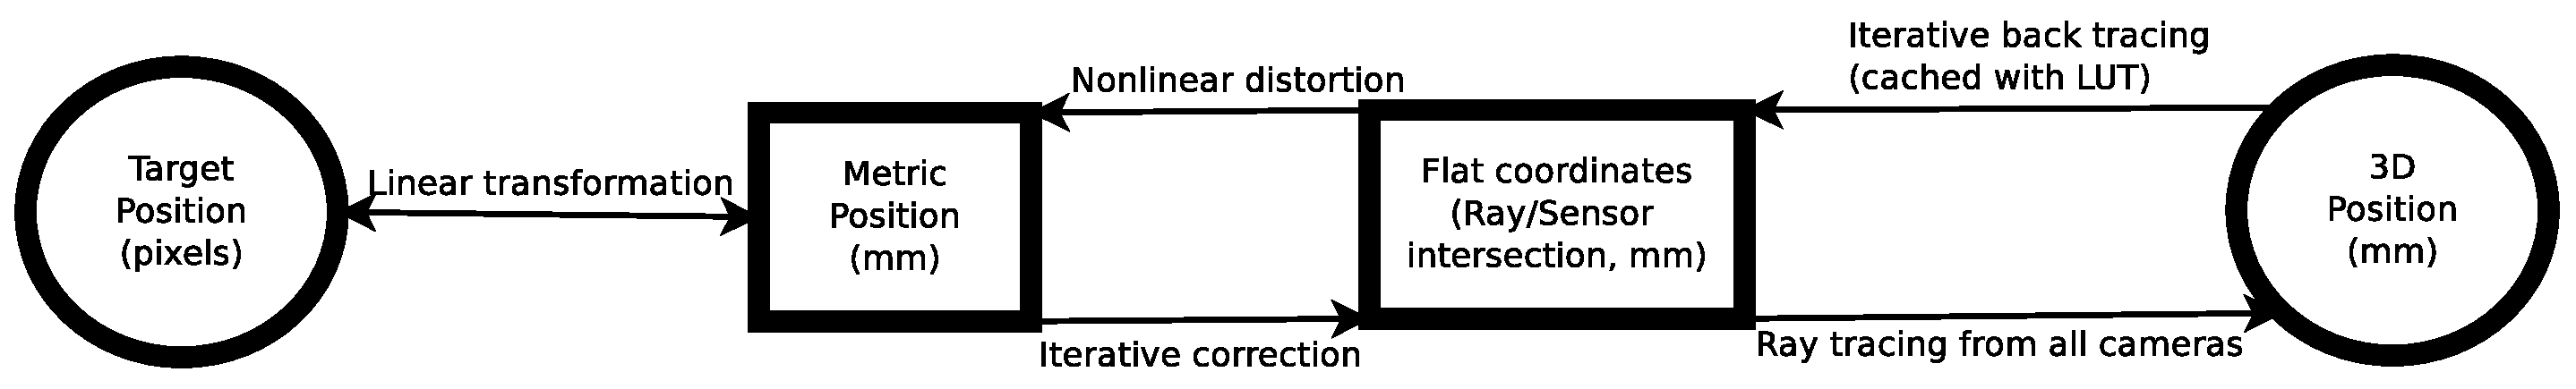
\includegraphics[width=1\columnwidth]{coord_transf}

\caption{Image coordinate systems\label{fig:Image-coordinate-systems}}


\end{figure}


The \emph{Pixel Coordinates} are the most obvious - they are the row
and column in the image data matrix. The origin is at the top-left
of the image, the y axis points down, the x axis points right, and
the units are pixels. The \emph{Metric Coordinates} are a simple linear
transformation of this system into one where the origin is at the
\emph{image}'s center point, y points up, x still points right, and
units are in millimeters. The unit conversion factor is based on the
pixel size in the sensor, so that the rightmost pixel x-coordinate
in the Metric system is half the sensor width in millimeters. The
sensor width and pixel size may be found in camera data sheets.

For example: For a sensor of $1280\times1024$ pixels (on the x and
y direction respectively), each $\unt{0.014}{\milli\metre}$ to a
side, Table \ref{tab:pixel-metric} shows the pixel and metric coordinates
of the image corners.

\begin{table}
\noindent \begin{centering}
\begin{tabular}{|c|c|c|}
\hline 
Corner & Pixel Coordinates $\left(x,y\right)$ & Metric coordinates $\left(x,y\right)$\tabularnewline
\hline 
\hline 
top left & 0,0 & -8.96,7.168\tabularnewline
\hline 
top right & 1280,0 & 8.96,7.168\tabularnewline
\hline 
bottom left & 0,1024 & -8.96,-7.168\tabularnewline
\hline 
bottom right & 1280,1024 & 8.96,-7.168\tabularnewline
\hline 
\end{tabular}
\par\end{centering}

\caption{Example of metric coordinates and the corresponding pixel coordinates.\label{tab:pixel-metric}}
\end{table}


Flat coordinates are a special case of the metric coordinates. They
arise from the fact that lens distortion and sensor shift lead to
a recorded image which is somewhat different than what would be seen
by an ideal pinhole camera as assumed by the simpler model. The metric
image coordinates denote coordinates of objects as seen by the camera.
The flat coordinates denote the position where an ideal camera would
see the same objects. 

The flat coordinates are what you receive from using the multimedia
code to trace back a ray from a known 3D position to its intersection
with the sensor plane. To get to the Metric system, you must first
add the sensor shift to the coordinates, then calculate the distorted
coordinates using the usual distortion formulas.

The reverse operation is to find a point on the image plane that,
when tracing a ray from the camera primary point through it, after
all refractions, will intersect the object represented by a given
Metric target coordinates. This operation appears mainly in calculating
average 3D position from ray intersections. To do this one must first
\emph{undistort} (or \emph{correct}) the Metric coordinates. This
is an inverse problem to that of distortion and is solved iteratively.
Then the sensor shift is subtracted from the result to yield the Flat
coordinates.

In the old 3DPTV code, with some exceptions, Pixel coordinates are
held in the \texttt{pix} arrays; Metric coordinates are in the \texttt{crd}
arrays; and Flat coordinates are in the \texttt{geo} arrays.

\bibliographystyle{plain}
\bibliography{refs}

\end{document}
